\chapter{Methodology}

\section{Some fundamental aspects of dynamical systems theory}

\subsection{Our dynamical systems and the uniqueness and existence of their solutions}
In this thesis we study dynamical systems described by a state variable $x = (x_1, x_2, \ldots, x_n)^T \in M $, where $M \subseteq \mathbb{R}^n$ is the state space, and $T$ denotes the transpose operation. The state variable is a point in this n-dimensional state space. In a continuous-time dynamical system, the state evolves according to the equation:
%
\begin{align}
    \dot{x}(t) = f(x(t))
    \label{eq:general-ds}
\end{align}

% where $f:M\to M$. Systems obeying Eq.~\ref{eq:general-ds} are deterministic: there is no randomness, no stochasticity, no noise. This means that, starting from one single state at time $t$, we can in principle describe the whole past and future evolution of the system. Furthermore, there is a lack of an explicit time dependence in $f$ - i.e., $\frac{\partial f_i}{\partial x_j} = 0 \; i,j=1, \ldots, n$. In this case, the dynamical system is said to be autonomous. 
where $f:M\to M$. Systems obeying Eq.~\ref{eq:general-ds} are deterministic: there is no randomness, no stochasticity, no noise. This means that, starting from one single state at time $t$, we can in principle describe the whole past and future evolution of the system. Furthermore, there is a lack of an explicit time dependence in $f$ - i.e., ${\partial f_i}/{\partial t} = 0$ for $i=1, \ldots, n$. In this case, the dynamical system is said to be autonomous. 

To obtain solutions to system \ref{eq:general-ds} we need to provide one state, which we typically call an initial condition $x_0 = x(0) \in \mathbb{R}^n$. The combination of $\dot{x} = f(x)$ with $x(0) = x_0$ defines an initial value problem. A fundamental theorem makes our lives studying this problem much easier. This is the theorem of existence and uniqueness of solutions. For $x \in \mathbb{R}^n$ and $f:\mathbb{R}^n\to\mathbb{R}^n$, it requires that $f$ is continuous and that all of its partial derivatives $\frac{\partial f_i}{\partial x_j}$, for $i, j = 1\ldots n$ are continuous in some open connected set $D \subset \mathbb{R}^n$. This basically means that it requires our function $f$ to be sufficiently smooth. Then, for initial conditions $x_0 \in D$, the initial value problem has a solution $x(t)$ on some time interval $(-\tau, \tau)$ about $t=0$, and the solution is unique! \cite{strogatz2002nonlinear} 

In state space, each solution describes a trajectory, a path, that goes through its initial condition $x_0$. The uniqueness of solutions implies that, within this time interval $(-\tau, \tau)$, different trajectories do not intersect in state space. This is a crucial property underlying all systems we study. 

A useful notation for the evolution of a continuous dynamical system is through the evolution operator $\Phi^t(x)$, which, informally defined, evolves the point $x$ forward $t$ time units. That is, $\Phi^t(x(0)) = x(t)$.

\subsection{The fate of linear dynamical systems}\label{method:linear-system}
Although trajectories do not cross, they can share the same fate, meaning they can converge to the region in state space. We can introduce this notion with a very simple mathematical example of a linear system. It has the form
% 
\begin{align}
    \dot{x}(t) = A x(t)
    \label{eq:linear}
\end{align}

where $A$ is a constant $(n \times n)$ matrix. %An example of a linear system if a simple harmonic oscillator, which is composed of a spring with constant $k$ connected to a body of mass $m$, whose position then changes according to $m\ddot{x} + kx = 0$. has to have friction here  

If the eigenvalues $\lambda_i \in \mathbb{C}$ of $A$ are all unique, its eigenvectors $v_i \in \mathbb{R}^n$ are linearly independent. Then, the general solution to this system can be written as Ref.~\cite{strogatz2002nonlinear}:
%
\begin{align}\label{eq:solution-linear}
    x(t) = \sum_{i=1}^n C_i e^{\lambda_i t} v_i.
\end{align}

Then, each initial condition determines the constant coefficients $C_i \in \mathbb{R}$. 
From Eq.~\ref{eq:solution-linear} we can already notice that the origin of the system, $ o = (0, \ldots, 0)^T$, is a solution. In fact, it is an equilibrium: $\dot{x} = f(o) = 0$. A trajectory on the origin does not change over time.

As we see from Eq. \ref{eq:solution-linear}, the behavior of trajectories depends on the eigenvalues $\lambda_i$ of the matrix $A$. We can classify the equilibrium at the origin based on these eigenvalues, as shown in Fig.~\ref{fig:method:equilibria-linear}. If the real parts of all the eigenvalues are negative, then all trajectories in state space converge to the origin as $t \to \infty$. In this case, the origin is said to be a stable equilibrium (Figs. \ref{fig:method:equilibria-linear}A-B). If at least one eigenvalue is negative, the trajectories diverge from the origin, which is then an unstable equilibrium (Figs.~\ref{fig:method:equilibria-linear}C-E). Stability here refers to the behavior of trajectories near the equilibrium. If it stable, nearby trajectories converge to the equilibrium - or, equivalently, small perturbations that take a trajectory away from the equilibrium will eventually go back to the equilibrium. If it is unstable, then nearby trajectories diverge from it.


Stable equilibria are the only attracting solution, or attractor, of linear systems. In this case, although different trajectories cannot not intersect, they all converge to the origin as $t \to \infty$. %This origin itself has no dynamics: the trajectory starting at the origin does not move. For this reason we say that the origin, the attractor in this system, is invariant: the set $\{o\}$ flows onto itself.  
In summary, the ultimate fate of linear systems is kind of boring: either trajectories end up at the origin or they diverge off to infinity. But the journey, the path that trajectories take before before the end, the \textit{transient dynamics}, is more interesting. As shown in Fig. \ref{fig:method:equilibria-linear}, this is dictated by the constellation of eigenvalues $\lambda_i$. For more details, the reader can refer to standard books on linear/nonlinear dynamics, such as Ref.~\cite{strogatz2002nonlinear}. 
%
\begin{figure*}
    \centering 
    \includegraphics[width=\textwidth]{equilibria-linear/hyperbolic-eq-2d.png}
    \caption{Hyperbolic equilibria in 2D linear systems. The title specifies the number of eigenvalues that are purely real negative $r_-$ or positive $r_+$, or that are complex with real part negative $c_-$ or positive $c_+$. The first row shows equilibria whose eigenvalues are purely real, while the second one shows equilibria with complex eigenvalues. In the first column, the equilibria are stable - they are the two possible attractors in linear systems. In the second column, we have a saddle-point for purely real eigenvalues. In the third column, the equilibria are completely unstable, known as repellers.  }
    \label{fig:method:equilibria-linear}
\end{figure*}




\subsection{The fate of nonlinear dynamical systems I: attractors}\label{method:nonlinear-I}
As just seen, stable equilibria are the only possible attractors in linear systems. Going beyond Eq.\ref{eq:linear}, nonlinear systems can have more interesting and complicated long-term dynamics (Fig.~\ref{fig:method:attractors-nonlinear}). Stable equilibria are still possible, as shown in Figs.\ref{fig:method:attractors-nonlinear}A-B. The system here is a conductance-based neuronal model following equations \cite{izhikevichbook}
%
\begin{align}
    &\dot{x} = \big(I - g_L (x_i - E_L)  
    - g_{Na} m_\infty(x_i) (x_i - E_{Na}) 
    -g_K y_i (x_i - E_K) \big)/C, \notag\\
    &\dot{y} = (n_\infty(x) - y_i) / \tau,
    \label{eq:inapk}
\end{align}

with all parameters and functions defined in detail in Chapter \ref{chap:multistability}. The input current $I$ is chosen to be $I=2.0$ so the system has excitable dynamics. Its state space is composed of a stable equilibrium, the only attractor, and two unstable equilibria, which create excitable dynamics. Excitability is a type of transient different than seen for linear systems. Some trajectories are forced to go on long excursions (excitations) before converging to the stable equilibrium. We study more about this again in Chapter \ref{chap:multistability}.

Besides equilibria, nonlinear systems can also have periodic solutions, also called limit cycles. They vary in time with a certain period $T$ (Fig.~\ref{fig:method:attractors-nonlinear}C) and correspond to closed curves in state space (Fig.~ \ref{fig:method:attractors-nonlinear}). The system used in this example is still the neuronal model of Eq.\ref{eq:inapk}, but with a different parameter $I=6$, which leads to the system now having a stable limit cycle. We see in this figure again an example of a long transient, with the trajectory initially going on a long excursion before converging to the limit cycle.

Not all curves in state space are closed, however. One can have quasiperiodic dynamics, in which trajectories never repeat exactly, although they might almost repeat. This is seen in Figs.~\ref{fig:method:attractors-nonlinear}E-F. Simulating the trajectory for longer times would fill up the figure more and more. Further, note the varying amplitude of the time series. The system in this example is the forced Van der Pol oscillator, 
%
\begin{align}
    &\dot{x} = v \\
    &\dot{v} = \mu (1-x^2)v - \alpha x + g \cos(\omega_f t),
    \label{eq:vanderpol},
\end{align}
with parameters $\mu=0.1$, $\alpha=1.0$, $g=0.5$, $\omega_f=\sqrt{3}$ taken from Ref.\cite{shukla2014a}.


Finally, one can also have chaotic attractors (Figs.\ref{fig:method:attractors-nonlinear}G-H). These solutions have a wild behavior that nearby trajectories tend to diverge at an exponential rate \cite{}. Despite this local divergence, however, the solutions remain bounded in space. 
In other words, systems with chaotic attractors are very sensitive to the initial conditions - small changes in initial conditions lead to trajectories that can look very different.  
% % Moreover, a chaotic attractor typically has a dense set of unstable periodic orbits embedded within it. These periodic orbits form the skeleton of the chaotic dynamics \cite{scholarppedia}
% The geometric structure of the solutions is very complicated, so proper rigorous analysis are often too difficult to perform. One important result, following the Poincaré-Bendixon Theorem, is that chaos is only possible in flows of dimension $3$ upwards (for maps, dimension $1$ already suffices) \cite{glendinning_1994, strogatz_2018}.
The system used to generate is shown as the Lorenz system, with equations 
%
\begin{align}
    &\dot{x} = \sigma. (y-x) \\ 
    &\dot{y} = x(\rho-z) - y \\ 
    &\dot{z} = x*y -\beta*z,
    \label{eq:lorenz}
\end{align}
and $\sigma = 10$, $\rho = 28$, $\beta = 8/3$. This chaotic attractor in particular has a shape that resembles a butterfly, with trajectories spending some time on one wing before switching to the other wing \cite{argyrisbook}. 



\begin{figure*}[htb!]
    \centering 
    \includegraphics[width=\textwidth]{attractors-nonlinear/attractors-nonlinear.png}
    \caption{Basic types of attractors in nonlinear dynamical systems. Each column shows respectively the state space and a time-series of a typical trajectory converging to a type of attractor. The first column corresponds to the neuronal model of Eq.\ref{eq:inapk} with $I=2.0$, which has excitable dynamics, converging to a stable equilibrium. The second column shows again the neuronal system of Eq.\ref{eq:inapk} but with $I=6.0$, when the attractor is now a stable limit cycle. The third column shows the system defined in Eqs.\ref{eq:vanderpol}, with a quasiperiodic attractor Finally, column four has an example of a chaotic trajectory on the Lorenz system (Eq.~\ref{eq:lorenz}).}
    \label{fig:method:attractors-nonlinear}    
\end{figure*}



Given now these examples, let us now define the terms we have used a bit more properly. 

% 
\subsection{Formalizing attractors and basins}
We have just presented examples of attractors, sets of points in state space to which trajectories eventually converge, and their basins of attraction, the regions containing those converging trajectories. Since in this thesis we will deal a lot with these concepts, we provide now an attempt at formalizing. The idea is to have the concepts clear in mind for later. In practice, we will only use the informal definition we just gave. In particular, the definition of attractor can vary considerably in the literature. Without attempting to claim any superiority, we attempt here to provide a definition that suits our studies.  

% As mentioned before, there are regions in state space wherein trajectories converge to a single common attractor. These are known as the basin of attraction $\mathcal{B}(A)$ of that attractor $A$. A common and intuitive mathematical definition of a basin is given in Ref.~\cite{milnor1985on}, which depends on the concept of the omega limit set $w(x)$ of a point $x$. The $\omega$-limit set of a point $x_0 \in M$ is defined as 
First, we define an omega limit set $w(x)$ of a point $x_0 \in M$ as \cite{milnor1985on}: 
% 
\begin{equation}
    \omega(x_0) = \{x: \forall\,T \;\forall \epsilon > 0\; \text{there exists } t > T \text{ such that } |f(x_0, t) - x| < \epsilon    \}.
\end{equation}

Consider a point $x \in\omega(x_0)$ in the $\omega$ limit set of $x_0$. Then, by definition, a trajectory that passes through $x_0$ comes arbitrarily close to $x$ infinitely often as $t$ increases. 

From this, we can define the \textit{basin of attraction} of a set $A$ as $\mathcal{B}(A) = \{x \in M: \omega(x) \subset A\}$. This only looks at the long-term behavior of trajectories; the transient dynamics could be anything, including the case that trajectories go very far from $A$, as long as they go back to it and stay there eventually. 
% If $\rho(A)$ is a smooth manifold but its dimension is smaller than the dimension of the state space $M$, then it simply the stable manifold of $A$ \cite{milnor1985on}.


% \subsection{Milnor attractor}\label{fundam:ssec:milnor-attractor}
Now to define an attractor, we first define a weaker (or, on the more optimistic side, a more general) version, called the \textit{Milnor attractor}. It is a useful concept when dealing with metastability. A set $A$ is a Milnor attractor if:
\begin{enumerate}
    \item Its basin of attraction $\mathcal{B}(A)$ has strictly positive measure (i.e., if $m(\mathcal{B}(A)) > 0$ ), where $m(S)$ denotes a measure equivalent to the Lebesgue measure of set $S$ \cite{milnor1985on}. This condition says that there is some probability that a randomly chosen point will be attracted to $A$ \cite{milnor1985on}.
    \item For any closed proper subset $A^\prime \subset A$, the set difference $\mathcal{B}(A) \setminus \mathcal{B}(A^\prime)$ also has strictly positive measure. This ensures that every part of $A$ plays an essential role - one cannot decompose $A$ into an attracting part and another part that does not attract \cite{milnor1985on, taylor2011attractors}. A closed set here means that it contains all its limit points. And proper means its non-empty.
\end{enumerate}

Furthermore, the Milnor attractor does not have to attract all the points in its neighborhood, and there can also be orbits that transiently go very far from the attractor, even if initially close, before eventually getting close to it. Further, it can in principle be composed into the union of two smaller Milnor attractors. To avoid these cases, we call a set $A$ an \textit{attractor} if
%
\begin{enumerate}
    \item $A$ is a Milnor attractor.
    \item $A$ contains an orbit that is dense in $A$. Basically, this means that the there is an orbit in $A$ that passes arbitrarily close to every point in $A$. This condition ensures that the attractor is not the union of two smaller attracting sets \cite{taylor2011attractors}. %It also ensures that orbits cannot escape from the attractor once they are in.
    \item There are arbitrarily small neighborhoods $U$ of $A$ such that $\forall x \in U$ one has $\Phi^t(x) \subset U  \; \forall t>0$ and such that $\forall y \in U$ one has $\omega(y) \subset \omega(x)$. That is, there are arbitrarily small neighborhoods around the attractor in which points inside stay inside and converge to $A$. This criterion is given in Ref.~\cite{broer2011dynamical}.
\end{enumerate}

\subsection{Invariant manifolds: structures that organize state space}

In Sec.~\ref{method:linear-system} we only considered the case when all the eigenvalues of the matrix $A$ in the linear system $\dot{x} = A x$ were positive. If one eigenvalue $\lambda_k$ is positive, then trajectories will diverge to infinity following the corresponding eigenvector $v_k$. When some eigenvalues are positive, and some are negative, the origin is a saddle-point. If all eigenvalues are positive, it is called a repeller.
Figure \ref{fig:method:equilibria-linear} shows examples of equilibria in 2D linear systems. Note that typical trajectories approach the saddle-point along the $y$-axis and then diverge along the $x$-axis. That is, for $t \to -\infty$, trajectories converge to the $y$-axis and for $t \to \infty$ they converge to the $x$-axis. The $y$-axis is called the stable manifold $\mathbb{W}^s(o)$ of the origin $o$ and the $x$-axis is the unstable manifold $\mathbb{W}^u(o)$ of the origin. We can define these manifolds
\begin{align}
&\mathbb{W}^s(o) = \{x \in M: \Phi^t(x) \to o \;\mathrm{as}\; t\to\infty\}, 
&\mathbb{W}^u(o) = \{x \in M: \Phi^t(x) \to o \;\mathrm{as }\; t\to -\infty\}.
\end{align}

Let us separate the eigenvectors $v_i$ into two parts: the ones with negative eigenvalues $v^-_1, \ldots, v^-_{n_s}$ and the ones with positive eigenvalues $v^+_1, \ldots, v^+_{n_u}$ . Then we can define the stable and unstable subspaces, respectively, as 
%
\begin{align}
    &\mathbb{E}^s = \mathrm{span}(v^-_1, \ldots, v^-_{n_s})
    &\mathbb{E}^u = \mathrm{span}(v^+_1, \ldots, v^+_{n_u})
\end{align}

For a linear system, the stable manifold of the origin coincides with the stable space $\mathbb{E}^s$ and the unstable manifold coincides with the unstable space.  In general, as in the example of the saddle-point, these manifolds act to organize the behavior of trajectories in state space.


These concepts can be extended for nonlinear systems. To do this, the first step is to think about the linearization of the nonlinear system. Suppose our nonlinear system of interest has an equilibrium $x^\star \in M$. It turns out that the behavior sufficiently close to this equilibrium is linear, despite the system globally being nonlinear \cite{saletan, glendinning}! To see this, we first move the origin of our system to $x^\star$ by defining a new variable $y(t) = x(t) - x^\star$. Then, 
%
\begin{align}
    \dot{y} = \dot{x} = f(y+x^\star) \equiv g(y)
\end{align}

where we define a convenience function $g(y)$. Expanding $g(y)$ around $y=0$ (i.e., around the equilibrium $x(t) = x^\star$) gives us 
%
\begin{align}
    \dot{y} = g(0) + J_g(0) y + \mathcal{O}(y^2),
\end{align}

where $J_g(y) = \frac{\partial g_i(y)}{\partial y_j}$ is the Jacobian of $g$. It is related to the Jacobian of $f$ by $J_g(y) = J_f(x)$, so $J_g(y=0) = J_f(x=x^\star)$. Since $g(0) = f(x^\star) = 0$, then if we are sufficiently close to the origin we can also ignore the terms $\mathcal{O}(y^2)$ and therefore we get 
%
\begin{align}
    \dot{y} = J_g(0) y.
\end{align}

That is, the behavior of the nonlinear system sufficiently close to the equilibrium is linear, with the constant matrix function being the Jacobian evaluated at the equilibrium! 

But the good news don't stop here! There is the Hartman-Grobman theorem, which basically shows that the state space near a hyperbolic equilibrium to the state space of the linearization. An equilibrium is hyperbolic if the eigenvalues of the Jacobian evaluated on it are all nonzero, i.e., if $\lambda_i \neq 0 \forall i=1,\ldots,n$. Topologically equivalent means that the linearized state space and the local state space near the equilibrium are distorted versions of each other. They can be bended and warped, but not ripped. In particular, closed orbits have to remain closed, and connections between saddle points have to remain \cite{strogatz2002nonlinear}. Mathematically, topologically equivalent means there is a homeomorphism (continuous deformation with continuous inverse) from one state space into the other; trajectories can be mapped from one to the other, and the direction of time is the same \cite{strogatz2002nonlinear}. 

Stating the theorem more formally, suppose a hyperbolic equilibrium $x^\star \in M$ such that $f(x^\star) = 0$ and such that all its eigenvalues are nonzero. Then, there is a neighborhood $N$ of $x^\star$ and a homeomorphism $h: N\to M$ such that \cite{argyrisbook}
\begin{itemize}
    \item $h(x^\star) = 0$
    \item the flow $\dot{x} = f(x)$ in $N$ is topologically conjugate to the flow of the linearization $\dot{y} = A y$ by the continuous map $y = h(x)$. Topologically conjugate basically meaning a change of coordinates in a topological sense.
\end{itemize}

This guarantees that the stability of the equilibrium is the same in both cases, so we can use the linearization to gain important insights about the stability of equilibria in the nonlinear system! 

What about the stable and unstable manifolds? In analogy to the linear case, we can define local stable and unstable sets near a neighborhood $U$ of an equilibrium $x^\star$ for the nonlinear system \cite{argyrisbook}:
% 
\begin{align}
&\mathbb{W}^s_\mathrm{loc}(x^\star) = \{x \in M: \Phi^t(x) \to o \;\mathrm{as}\; t\to+\infty\  \mathrm{and}\; \Phi^t(x) \in U \;\forall t \geq 0\}, \\
&\mathbb{W}^u_\mathrm{loc}(x^\star) = \{x \in M: \Phi^t(x) \to o \;\mathrm{as }\; t\to -\infty\ \mathrm{and}\; \Phi^t(x) \in U \;\forall t\leq 0 \}.
\end{align}

Herein comes the stable manifold theorem. It states that, for a hyperbolic equilibrium $x^\star$:
\begin{itemize}
    \item The local stable set $\mathbb{W}^s_\mathrm{loc}(x^\star)$ is a smooth manifold whose tangent space has the same dimension $n_s$ as the stable space $\mathbb{E}^s$ of the linearization of $f$ at $x^\star$. $\mathbb{W}^s_\mathrm{loc}(x^\star)$ is also tangent to $\mathbb{E}^s$ at $x^\star$.
    \item The local unstable set $\mathbb{W}^u_\mathrm{loc}(x^\star)$ is a smooth manifold whose tangent space has the same dimension $n_u$ as the unstable space $\mathbb{E}^u$ of the linearization of $f$ at $x^\star$. $\mathbb{W}^u_\mathrm{loc}(x^\star)$ is also tangent to $\mathbb{E}^u$ at $x^\star$.
\end{itemize}

The homeomorphism guaranteed by the Hartman-Grobman theorem maps $\mathbb{W}^s_\mathrm{loc}(x^\star)$ into $\mathbb{E}^s$ and $\mathbb{W}^u_\mathrm{loc}(x^\star)$ into $\mathbb{E}^u$ one-to-one, as shown in Fig. XX. Further, the stable manifold theorem guarantees that $\mathbb{E}^s$ and $\mathbb{E}^u$ actually approximate the local manifolds $\mathbb{W}^s_\mathrm{loc}(x^\star)$ and $\mathbb{W}^u_\mathrm{loc}(x^\star)$, respectively \cite{argyrisbook}. As a consequence, we get the behavior illustrated in \figref{fig:method:invariantmanifolds}

The manifolds we just looked at are defined for a local neighborhood $U$ around the equilibrium. We can extend them towards the whole of state space by defining global manifolds as:
\begin{align}
    \mathbb{W}^s(x^\star) = \bigcup_{t\leq 0} \Phi^t(\mathbb{W}^s_\mathrm{loc}(x^\star)) \\
    \mathbb{W}^u(x^\star) = \bigcup_{t\geq 0} \Phi^t(\mathbb{W}^u_\mathrm{loc}(x^\star))
    \label{eq:global-manifolds}
\end{align}

That is, the global stable manifold is obtained by integrating the local stable manifold backwards, looking at where the trajectories on it came from. For the unstable manifold, we integrate the local unstable manifold forwards, to see where it goes to. 

An important fact about the local and global manifolds that follows from their definitions is that they are invariant: trajectories starting on these manifolds stay on them forever \cite{argyrisbook}.
Furthermore, the uniqueness of solutions prohibits certain crossings of manifolds: stable manifolds of two distinct equilibria cannot cross, unstable manifolds of two distinct equilibria also cannot, and the same manifold cannot cross itself - otherwise, where the crossing points would have to obey two distinct paths! Meanwhile, stable and unstable manifolds, either of the same equilibrium or of two different equilibria can cross. 

As mentioned before, these manifolds usually play a big role in organizing state space. As we will see in Chapter \ref{chap:multistability}, they can organize the transient dynamics of systems. There, we study a dynamical system wherein certain trajectories are forced to go on long excursions before converging to the stable equilibrium, the only attractor in state space (see Figs.\ref{fig:method:attractors-nonlinear}A-B). As explained there, this long excursion is generated by the arrangement of the invariant manifolds of the saddle-point that exists in state space. The invariant manifolds can also organize the long-term behavior of systems: the next section briefly shows how stable manifolds of unstable equilibria can act as the boundary separating two basins of attraction.


\begin{figure}
    \centering
    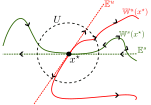
\includegraphics[width=0.6\textwidth]{global-manifolds/global-manifolds.png}
    \caption{Invariant manifolds of saddle point $x^\star$. The local stable $\mathbb{W}^s_\mathrm{loc}(x^\star)$ and unstable $\mathbb{W}^u_\mathrm{loc}(x^\star)$ manifolds of the saddle point $x^\star$ respectively can be associated with the stable $\mathbb{E}^s$ and unstable $\mathbb{E}^u$ subspaces and become tangent to them near the saddle. This follows from the Hartman-Grobman and the stable manifold theorems. The global stable $\mathbb{W}^s(x^\star)$ and unstable $\mathbb{W}^u(x^\star)$ manifolds extend the definition of the local manifolds beyond the neigborhood $U$.  Figure is inspired by Fig.~6.2.4 from Ref.~\cite{argyrisbook}.}
    \label{fig:method:invariantmanifolds}
\end{figure}

\subsection{The fate of nonlinear dynamical systems II: multistability and basins of attraction}
% Linear system are monostable: they can have only one attractor. If we now move to nonlinear systems, the situation is different. Now, trajectories can have multiple distinct fates, multiple attractors. To which attractor a trajectory goes to depends on where it starts. In a multistable system, the state space is then divided into distinct regions, wherein trajectories starting on each region go to their corresponding attractor. A simple and intuitive example is that of a ball on a certain landscape with hills and valleys. The ball of course rolls downhill and, due to friction, it eventually stops at one of the valleys.
In Sec.~\ref{method:nonlinear-I} we saw that the ultimate fate of nonlinear systems, their attractors, can be much more complicated than that of linear ones. Not only are the attractors themselves complicated, but they can also coexist in state space. If there are two coexisting attractors, this means that the state space will be separated into three regions: the basin of attraction of attractor one, the basin of attractor two, and the boundary between them. Usually, the basin boundary is formed by stable manifolds of saddle-type objects: saddle-points, saddle-limit-cycles, and even chaotic saddles! \cite{pisarchik}. Figure~\ref{fig:bistability-duffing} illustrates this for a relatively simple system with two stable equilibria, where the basin boundary is the stable manifold of the saddle-point in the middle. This system is known as the Duffing oscillator: 

\begin{align}
    &\dot{x} = v\\
    &\dot{v} = -(-kx + cv + lx^3)/m,
\end{align}

with $k = 1$, $c=0.5$, $l=1$, $m=1$. This system represents a ball of mass $m$ rolling downhill at position $x$ and velocity $v$ on a quartic potential landscape of the form $U(x) = -lx^4/4 - kx^2/2$ with a friction term $-cv$. Following the definition of global manifolds in Eq.\ref{eq:global-manifolds}, these global manifolds are essentially obtained by integrating trajectories starting on the local manifolds of the saddle-point. 
%
\begin{figure}[htb!]
    \centering 
    \includegraphics[width=0.6\columnwidth]{duffing-bistability.png}
    \caption{Bistability in Duffing model. Two stable equilibria (white square and circle) are shown with their respective basins of attraction in two shades of purple. The global stable and unstable manifolds of the saddle-point (black point) in the middle are also shown as green and red lines respectively. The global stable manifold of the saddle coincides with the boundary between the basins.}
    \label{fig:bistability-duffing}
\end{figure}


In this thesis we study two examples of multistability occuring in networked systems. In Chapter \ref{chap:malleability} we study networks of Kuramoto units, and see there the coexistence of multiple attractors depending on how strongly the units are interacting. We also see how this multistability impacts the sensitivity of the system to small changes in parameters of the units. Later, in Chapter \ref{chap:multistability} we study how multistability arises when two excitable neurons are coupled together diffusively. Both studies require that we find the attractors in the systems. This is what we deal with in the next section.

\subsection{How to find attractors}


% \section{Bifurcations}
% Depending on the parameters, a dynamical system may have all three of the above attractors, stable or not, simultaneously or not. When the system changes drastically its qualitative behavior as one parameter is changed, we say a bifurcation has taken place. This can lead, for example, from an equilibrium to a periodic orbit. 
% 
% As we have seen from the linear stability analysis, if the stationary point is hyperbolic, then the local behavior is determined by the linearized flow. Following from this is that small perturbations from this point are also hyperbolic.
% % hyperbolic point, for which all the eigenvalues of the linearized flow have nonzero real parts
% Therefore, we have bifurcations only for non-hyperbolic points (i.e. points with at least one eigenvalue that is zero or purely imaginary).
% 
% Now we describe some bifurcations that are relevant for this dissertation. This is done for equilibria (fixed points), but the general considerations also apply for periodic orbits.
% 
% 
% \subsection{Saddle-node (fold) bifurcation}
% In a saddle-node bifurcation two equilibria (one stable and the other unstable) coalesce and annihilate each other. Therefore, this bifurcation deals with the creation (and destruction) of stable and unstable equilibria. In this case, one equilibrium had a negative eigenvalue and the other has a positive eigenvalue before bifurcation. At the bifurcation, these values reach $0$ and later the points are destroyed \cite{strogatz_2018}. 
% This scenario also occurs for periodic orbits (e.g. limit cycles).
% 
% Neurons passing through this bifurcation are of type II excitability (cf. \chapref{chap:neuronal_models}), the exception being if the bifurcation occurs on an invariant circle (a saddle-node on invariant circle bifurcation), where the neuron has type I excitability \cite{izhikevich_2007}.
% 
% \subsection{Andronov-Hopf}
% In an Andronov-Hopf bifurcation, a small-amplitude limit cycle is born from an equilibrium: it appears when the equilibrium disappears. In a supercritical bifurcation, the limit cycle is born stable (and the equilibrium loses its previous stability). In a subcritical, the inverse happens: the limit cycle is born unstable and the equilibrium gains stability. In this case, the Jacobian has a pair of complex eigenvalues whose real part becomes zero at the bifurcation.
% 
% Neurons passing through this bifurcation are of type II excitability \cite{izhikevich_2007}.
% 
% \subsection{Homoclinic bifurcations}
% The homoclinic bifurcations also describe the appearance (or disappearance) of limit cycles (two-dimensional periodic orbits). The bifurcation is supercritical if the limit cycle is stable and supercritical if unstable. In the supercritical case, before the bifurcation there is a saddle and a stable limit cycle. At the bifurcation, these two touch each other, thereby making a homoclinic orbit (connecting the saddle to itself). After the bifurcation, the homoclinic orbit disappears (and the limit cycle already disappeared) and only the saddle remains. 
% In the subcritical case the behavior is similar, but the limit cycle is unstable.
% 
% An important point is that the homoclinic orbit has infinite period (or zero frequency), so neurons passing through this bifurcation are of type I excitability \cite{izhikevich_2007}.
% 
% 
% \subsection{Period-doubling (or flip) bifurcation}
% This bifurcation deals with the destruction of a periodic orbit of period $T$ and appearance of another of period $2T$.
% A cascade of period-doublings often occurs, leading to chaotic behavior \cite{ott_2002}. The inverse can also happen, leading from chaos to periodic behavior.
% 
